\label{chap.5}
\section{What this stage has to do}
Stage 2 takes the recent daily weather of a district and forecasts the coming days. Its output feeds the season summary (Stage 3): to judge whether the current season is heading into a dry spell or a delayed onset, the system needs both the weather observed so far and a view of the days ahead. The forecasting model has to work without calling an external weather service, so it is trained only on the district's own 26-year record.

Of all the weather variables, \textbf{rainfall} matters most here. Every condition in the contingency plans (delayed onset, dry spell, terminal drought, excess rain) is defined by rainfall, and rainfall is the main weather driver of rainfed crop yield. The project therefore uses a model designed specifically for daily rainfall, the \textbf{two-stage hurdle model}, as its \textbf{main forecasting model}, used one per district throughout the pipeline. Four other well-known approaches, an LSTM network, SARIMA, XGBoost and a Temporal Fusion Transformer, were trained on the same data as a \textbf{comparative study}, to check that the choice of the hurdle model is justified.

One rule applies to every model in this chapter: a forecast may use only information that would really be available on the day the forecast is made.

\section{Why daily rainfall needs a special model}
Daily rainfall behaves very differently from smooth variables such as temperature (Figure~\ref{fig:raindist}):
\begin{itemize}
	\item \textbf{Most days are dry.} In every district about 62--64\% of days have no measurable rain (0.25\,mm or less), and 80--83\% have less than 2.5\,mm, the India Meteorological Department's threshold for a "rainy day".
	\item \textbf{The rain that does fall is highly skewed.} On rainy days the median amount is only about 2--3\,mm, yet the heaviest 10\% of rainy days deliver about 42--44\% of all the rain.
\end{itemize}
A model that predicts rainfall as one continuous number, and is trained to keep its average error small, learns a poor compromise: it predicts "a little rain" on almost every day. That is never badly wrong on dry days, but it blurs the difference between dry and wet days and badly under-predicts heavy rain. Both are exactly what a drought system needs to get right.

\begin{figure}[H]
	\centering
	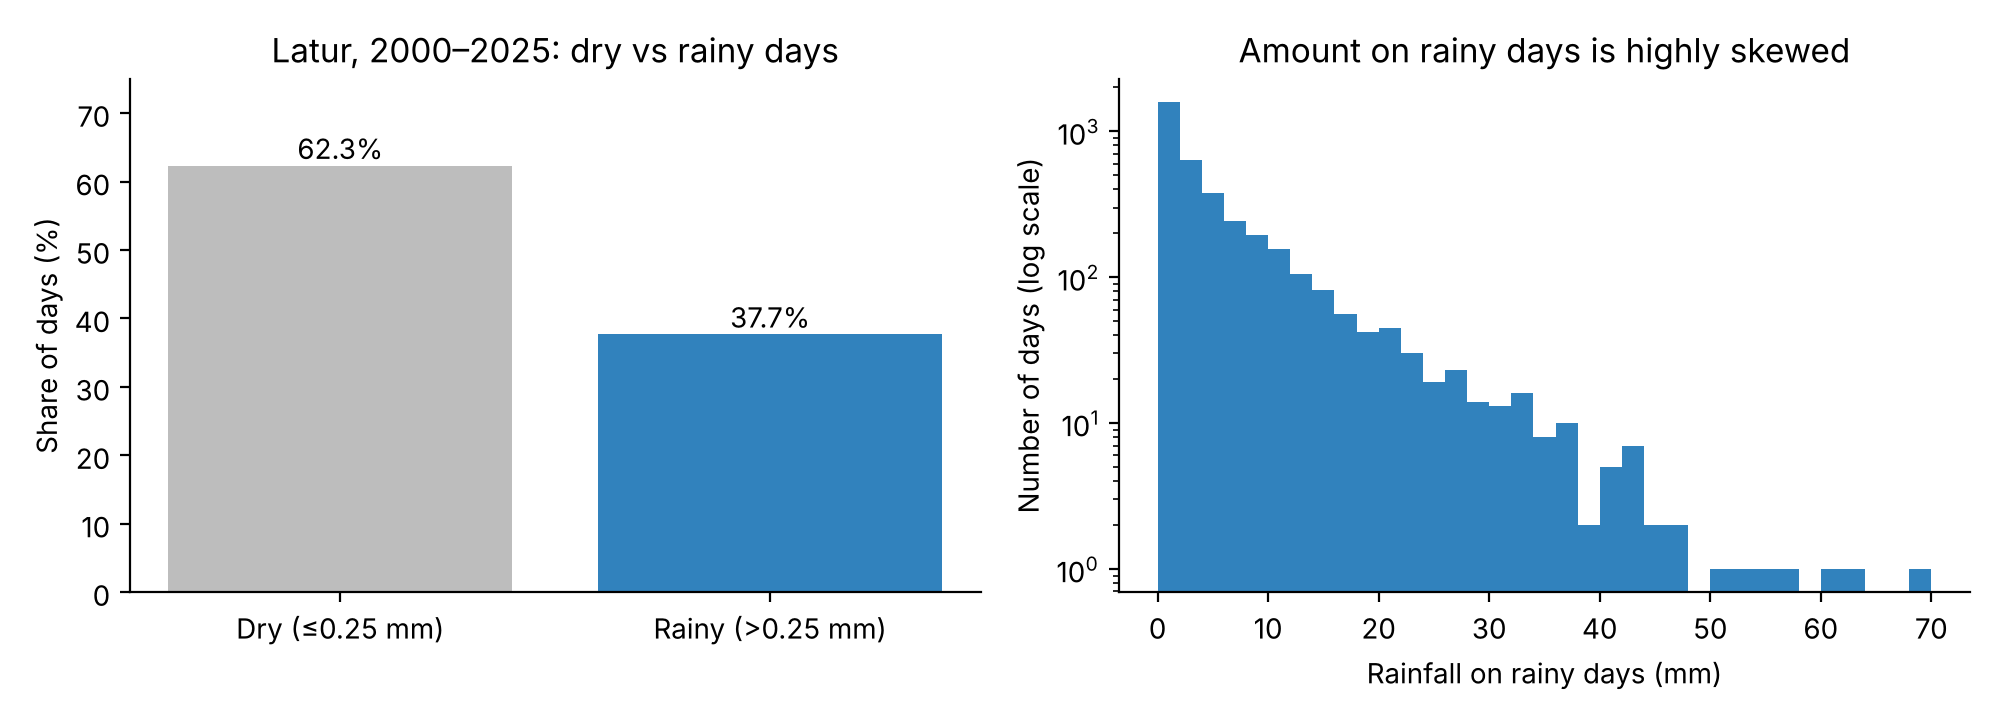
\includegraphics[width=\textwidth]{rain_distribution.png}
	\caption{Daily rainfall in Latur, 2000--2025. Left: about 62\% of days are dry. Right: rainy-day amounts are heavily skewed (note the log scale). The other four districts look the same.}
	\label{fig:raindist}
\end{figure}

Statisticians have long modelled such variables in two parts: first \emph{whether} the event happens, then \emph{how large} it is given that it happens \cite{cragg1971some,mullahy1986specification}. Classical daily-rainfall models do the same, pairing a wet/dry occurrence process with a separate distribution for the amount \cite{stern1984model}. The hurdle model follows this idea.

\section{Evaluation set-up}

\subsection{Chronological split}
Weather is a time series, so data are never shuffled; every model is trained on the past and tested on a later period it has never seen. For the hurdle model the split is made on the date being forecast (the \emph{target} date):
\begin{itemize}
	\item \textbf{Test:} target dates from 1 January 2022 onwards (about 1,718 days per horizon); all results below are on this period;
	\item \textbf{Validation:} the 365 days before the test period;
	\item \textbf{Training:} everything earlier, from 2000.
\end{itemize}

\subsection{Metrics}
For $n$ test days with observed values $y_t$, forecasts $\hat{y}_t$ and observed mean $\bar{y}$:
\begin{align}
	\text{RMSE} &= \sqrt{\frac{1}{n}\sum_{t=1}^{n}(y_t-\hat{y}_t)^2}, \qquad
	\text{MAE} = \frac{1}{n}\sum_{t=1}^{n}\lvert y_t-\hat{y}_t\rvert, \\
	R^2 &= 1-\frac{\sum_{t}(y_t-\hat{y}_t)^2}{\sum_{t}(y_t-\bar{y})^2}.
\end{align}
RMSE and MAE are in millimetres; RMSE punishes large misses more heavily. $R^2$ is unit-free: 1 means perfect, 0 means no better than always predicting the test-period average, and negative values mean worse than that. For daily rainfall a few heavy days dominate the sum of squares, so even a useful model has a modest $R^2$.

\section{The hurdle model (main model)}

\subsection{Structure}
For each district and each forecast horizon $h \in \{1,2,3\}$ days, the model has two parts (Figure~\ref{fig:hurdle}):
\begin{enumerate}
	\item \textbf{Hurdle 1, the rain gate.} A gradient-boosted classifier estimates the probability $p$ that day $t+h$ will have more than 0.25\,mm of rain.
	\item \textbf{Hurdle 2, the rain depth.} A gradient-boosted regressor, trained only on rainy days, predicts $\log(1+\text{rainfall})$ on day $t+h$. Working on the log scale tames the skew of heavy events.
\end{enumerate}
The forecast combines the two:
\begin{equation}
	\hat{y}_{t+h} =
	\begin{cases}
		\exp\big(g_h(\mathbf{x}_t)\big) - 1 & \text{if } p_h(\mathbf{x}_t) > \tau,\\
		0 & \text{otherwise,}
	\end{cases}
	\qquad \tau = 0.35,
\end{equation}
where $\mathbf{x}_t$ are the features available on forecast day $t$, $p_h$ is the gate and $g_h$ the depth model. The threshold $\tau = 0.35$ is set below 0.5 on purpose: because rainy days are the minority, a gate that waited for 50\% certainty would miss too many of them. Training separate models for each horizon (\emph{direct} multi-step forecasting) avoids feeding one day's forecast into the next, which would compound errors.

\begin{figure}[H]
\centering
\resizebox{\textwidth}{!}{%
\begin{tikzpicture}[
  font=\sffamily\small,
  box/.style={draw, rounded corners, minimum width=3.4cm, minimum height=1.0cm, align=center},
  arr/.style={-{Stealth[length=2.2mm]}, thick}
]
\node[box, fill=gray!12] (x) {Features known on\\forecast day $t$};
\node[box, fill=blue!8, right=1.4cm of x] (g) {Hurdle 1: rain gate\\$p$ = P(rain on $t{+}h$)};
\node[draw, diamond, aspect=2, fill=yellow!15, right=1.2cm of g, align=center, inner sep=1pt] (d) {$p > 0.35$?};
\node[box, fill=green!12, above right=0.3cm and 1.0cm of d] (r) {Hurdle 2: rain depth\\$\log(1+y)$ regressor};
\node[box, fill=gray!8, below right=0.3cm and 1.0cm of d] (z) {Forecast = 0 mm};
\node[box, fill=green!6, right=0.9cm of r] (o) {Forecast =\\$e^{g}-1$ mm};
\draw[arr] (x) -- (g); \draw[arr] (g) -- (d);
\draw[arr] (d.north) |- node[pos=0.25, left]{yes} (r.west);
\draw[arr] (d.south) |- node[pos=0.25, left]{no} (z.west);
\draw[arr] (r) -- (o);
\end{tikzpicture}}
\caption{The two-stage hurdle model. One gate and one depth model are trained for each district and each horizon $h = 1, 2, 3$ days.}
\label{fig:hurdle}
\end{figure}

\subsection{Features}
Every feature is computed only from data available on the forecast day $t$; rolling rainfall statistics end on the day \emph{before} $t$, so they never include the rain being predicted. The 21 features are:
\begin{itemize}
	\item \textbf{Season:} $\sin(2\pi d/365.25)$ and $\cos(2\pi d/365.25)$ of the day of year $d$, which tell the model where it is in the monsoon cycle and place 31 December next to 1 January;
	\item \textbf{Recent rain:} rainfall 1, 2 and 3 days earlier; mean rainfall over the previous 3, 7 and 14 days; maximum rainfall in the previous 3 days;
	\item \textbf{Moisture and pressure tendency:} humidity and pressure on the previous day and their day-to-day change; a falling pressure and rising humidity often precede rain;
	\item \textbf{Current conditions:} relative humidity, surface pressure, mean, maximum and minimum temperature, wind speed, solar radiation and dew point.
\end{itemize}

\subsection{Training settings}
Both parts use scikit-learn's histogram-based gradient boosting \cite{pedregosa2011scikit}: the gate with 250 boosting iterations and a learning rate of 0.04, the depth model with 350 iterations and a learning rate of 0.03, both with L2 regularisation of 0.1 and a fixed random seed. All settings live in one configuration file (Appendix~\ref{app:config}). Training needs no GPU and runs quickly on an ordinary laptop CPU, which makes regular retraining practical (Chapter~\ref{chap.7}).

\subsection{Model development: from nowcast to forecast}
\label{sec:leak}
The first version of the hurdle model also used physically motivated features (temperature range, dew-point spread, wind shear, vapour pressure deficit and a moisture-flux proxy) and a rule that set rainfall to zero when the air was clearly too dry. It scored very highly, with $R^2$ between 0.79 and 0.94. A careful review while building the MLOps pipeline showed why: its rolling rainfall features included the day being predicted, its humidity and temperature inputs were from that same day, and its target was same-day rainfall. In other words, it estimated today's rain from today's weather, a \emph{nowcast}, and was partly told the answer. This is a classic case of \emph{data leakage} \cite{kaufman2012leakage}. Figure~\ref{fig:hurdlev1} shows the symptom: the predicted series traces the observed one almost perfectly and with no delay, which no genuine forecast of daily rain can do.

\begin{figure}[H]
	\centering
	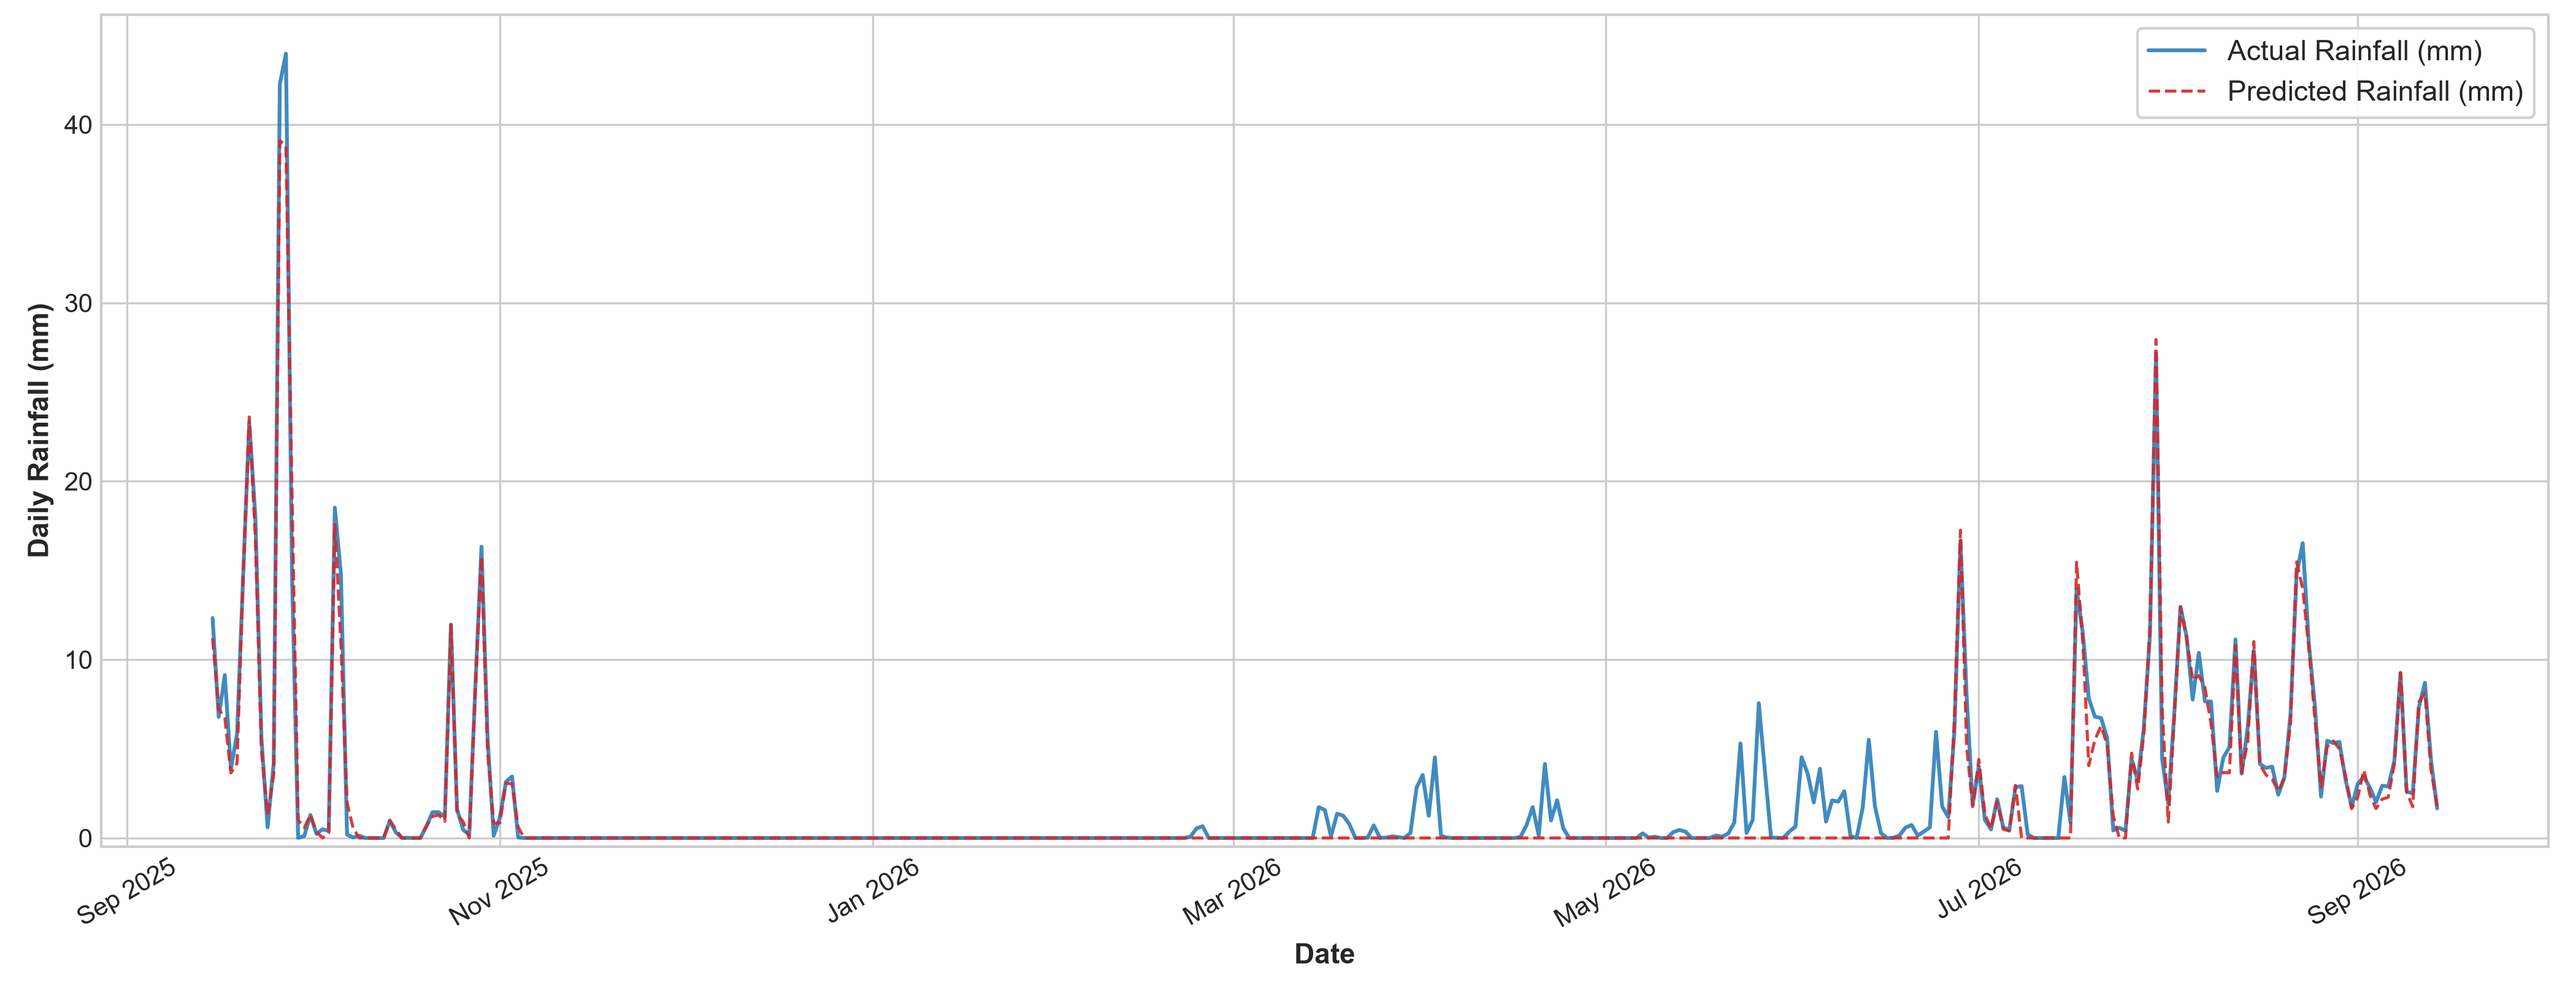
\includegraphics[width=\textwidth]{hurdle_v1_latur.png}
	\caption{First (same-day) version of the hurdle model, Latur, one-year validation window ($R^2 = 0.94$, RMSE 1.17\,mm, MAE 0.51\,mm). Because its inputs included the same day's rainfall, it reproduces the observed series almost exactly; it is a nowcast, not a forecast. The corresponding values for the other districts were $R^2$ 0.92 (Ahmednagar), 0.94 (Beed), 0.88 (Osmanabad) and 0.79 (Solapur).}
	\label{fig:hurdlev1}
\end{figure}

The model was therefore rebuilt as a genuine forecaster: features shifted so they end before the forecast day, targets moved $h$ days ahead, separate models per horizon, and the split made on the target date. All results in this chapter are for this corrected version, which is the one used in the project.

\subsection{Results}
Table~\ref{tab:hurdle} gives the test results for all five districts and all three horizons.

\begin{table}[H]
	\centering
	\caption{Hurdle model: rainfall forecast test results (target dates from 2022 onward)}
	\label{tab:hurdle}
	\small
	\begin{tabular}{lccccccccc}
		\toprule
		& \multicolumn{3}{c}{\textbf{Day +1}} & \multicolumn{3}{c}{\textbf{Day +2}} & \multicolumn{3}{c}{\textbf{Day +3}} \\
		\cmidrule(lr){2-4}\cmidrule(lr){5-7}\cmidrule(lr){8-10}
		\textbf{District} & $R^2$ & RMSE & MAE & $R^2$ & RMSE & MAE & $R^2$ & RMSE & MAE \\
		\midrule
		Ahmednagar & 0.151 & 7.09 & 1.62 & 0.103 & 7.29 & 1.74 & 0.072 & 7.41 & 1.80 \\
		Beed       & 0.259 & 4.74 & 1.62 & 0.190 & 4.96 & 1.77 & 0.147 & 5.08 & 1.77 \\
		Latur      & 0.289 & 4.50 & 1.80 & 0.186 & 4.81 & 1.99 & 0.154 & 4.91 & 2.04 \\
		Osmanabad  & 0.261 & 4.72 & 1.89 & 0.173 & 4.99 & 2.04 & 0.134 & 5.10 & 2.10 \\
		Solapur    & 0.282 & 4.12 & 1.59 & 0.150 & 4.49 & 1.73 & 0.106 & 4.60 & 1.82 \\
		\bottomrule
	\end{tabular}
	\\[2pt]
	\footnotesize RMSE and MAE in mm/day.
\end{table}

\begin{figure}[H]
	\centering
	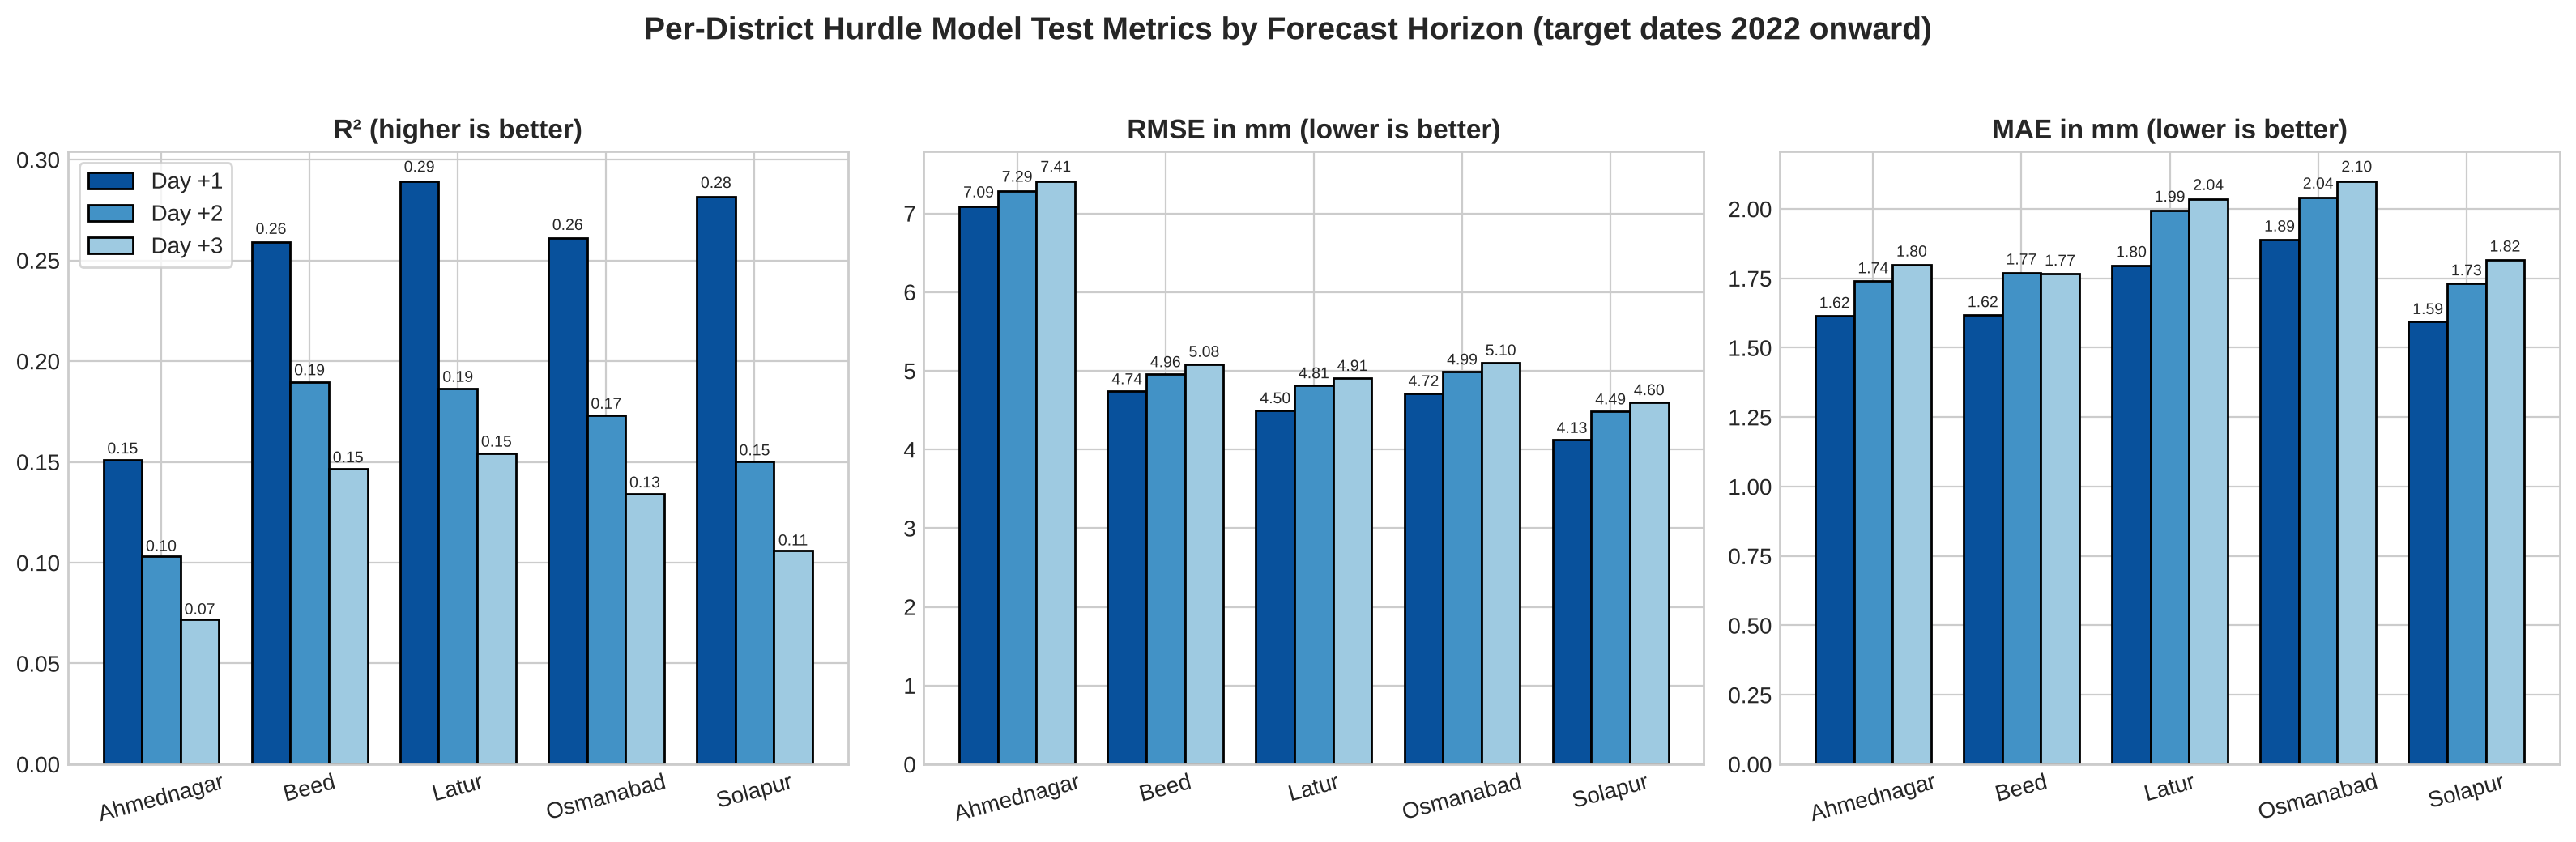
\includegraphics[width=\textwidth]{hurdle_metrics_summary.png}
	\caption{Hurdle model test metrics for each district and forecast horizon.}
	\label{fig:hurdlemetrics}
\end{figure}

\begin{itemize}
	\item \textbf{One day ahead}, the model explains 26--29\% of the day-to-day variation in rainfall in four of the five districts, with a typical error (MAE) of 1.6--1.9\,mm.
	\item \textbf{Skill falls with lead time}, to 0.07--0.15 by day 3. This is expected for point rainfall in a monsoon climate: whether it rains on a particular day a few days ahead is hard to predict from local history alone.
	\item \textbf{Ahmednagar is the hardest district.} Its RMSE is much larger because its record contains a few extreme events (one day exceeds 250\,mm) that dominate the squared error.
\end{itemize}

\paragraph{How well the gate separates dry and rainy days.} Because the drought rules in the plans depend on runs of dry days, the most important job of the model is to say correctly whether a day will be dry or rainy. Figure~\ref{fig:gate} evaluates Hurdle~1 on its own. One day ahead it classifies 84--88\% of days correctly and detects 89--92\% of rainy days; by day 3 accuracy is still 81--86\% and 84--87\% of rainy days are caught. About one in five of its "rain" calls turns out dry (18--26\% false alarms), which is the price of the deliberately low threshold $\tau = 0.35$: the gate prefers to catch rainy days, because a missed rainy day would wrongly extend a dry-spell count.

\begin{figure}[H]
	\centering
	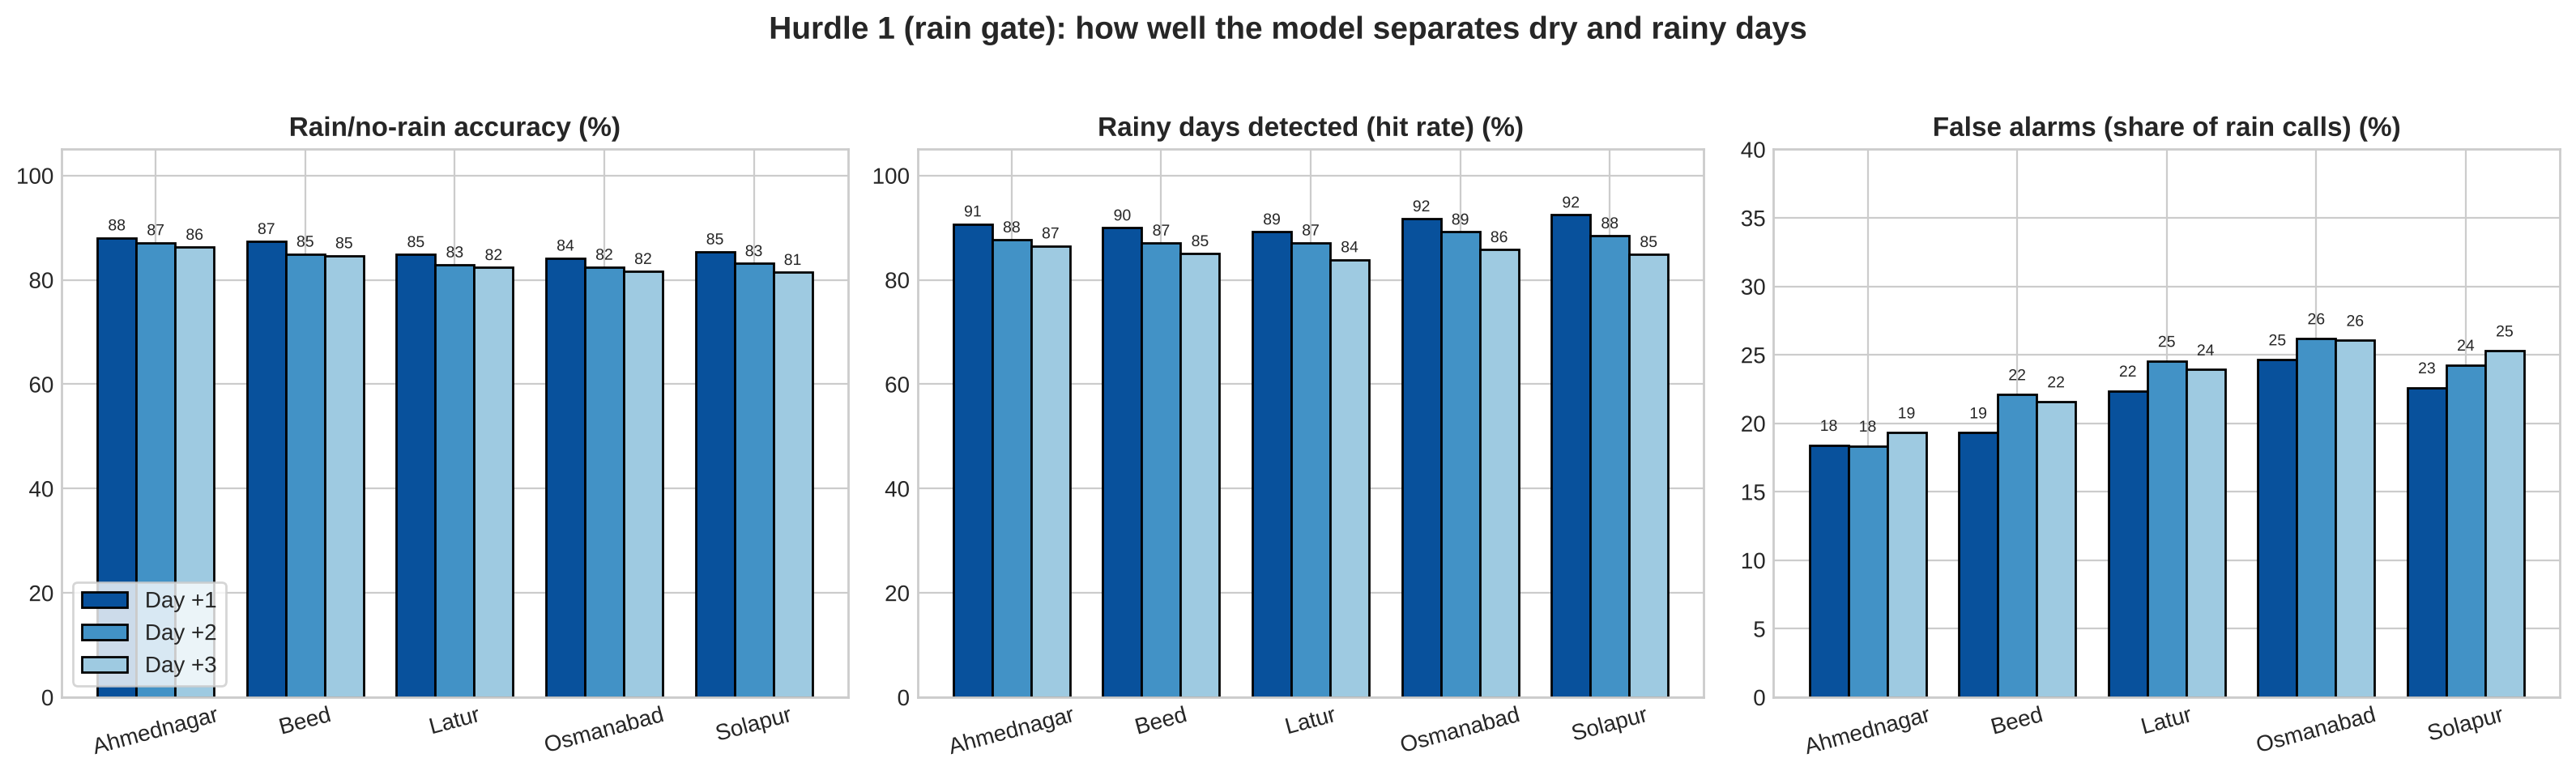
\includegraphics[width=\textwidth]{hurdle_gate_performance.png}
	\caption{Rain gate (Hurdle 1) on the test period: overall accuracy, share of rainy days detected, and share of rain forecasts that turned out dry.}
	\label{fig:gate}
\end{figure}

\paragraph{Forecasts over time.} Figure~\ref{fig:hurdleall} shows the one-day-ahead forecasts for all five districts over the last twelve months of the test period, and Figure~\ref{fig:hurdlelatur} zooms into the 2025 Kharif season in Latur. The model correctly keeps forecasts at zero through the dry months, and during the monsoon it follows wet and dry spells, but it rounds off the peaks: a 40\,mm day is typically forecast as 5--15\,mm, and the three-day-ahead forecast is smoother still.

\begin{figure}[H]
	\centering
	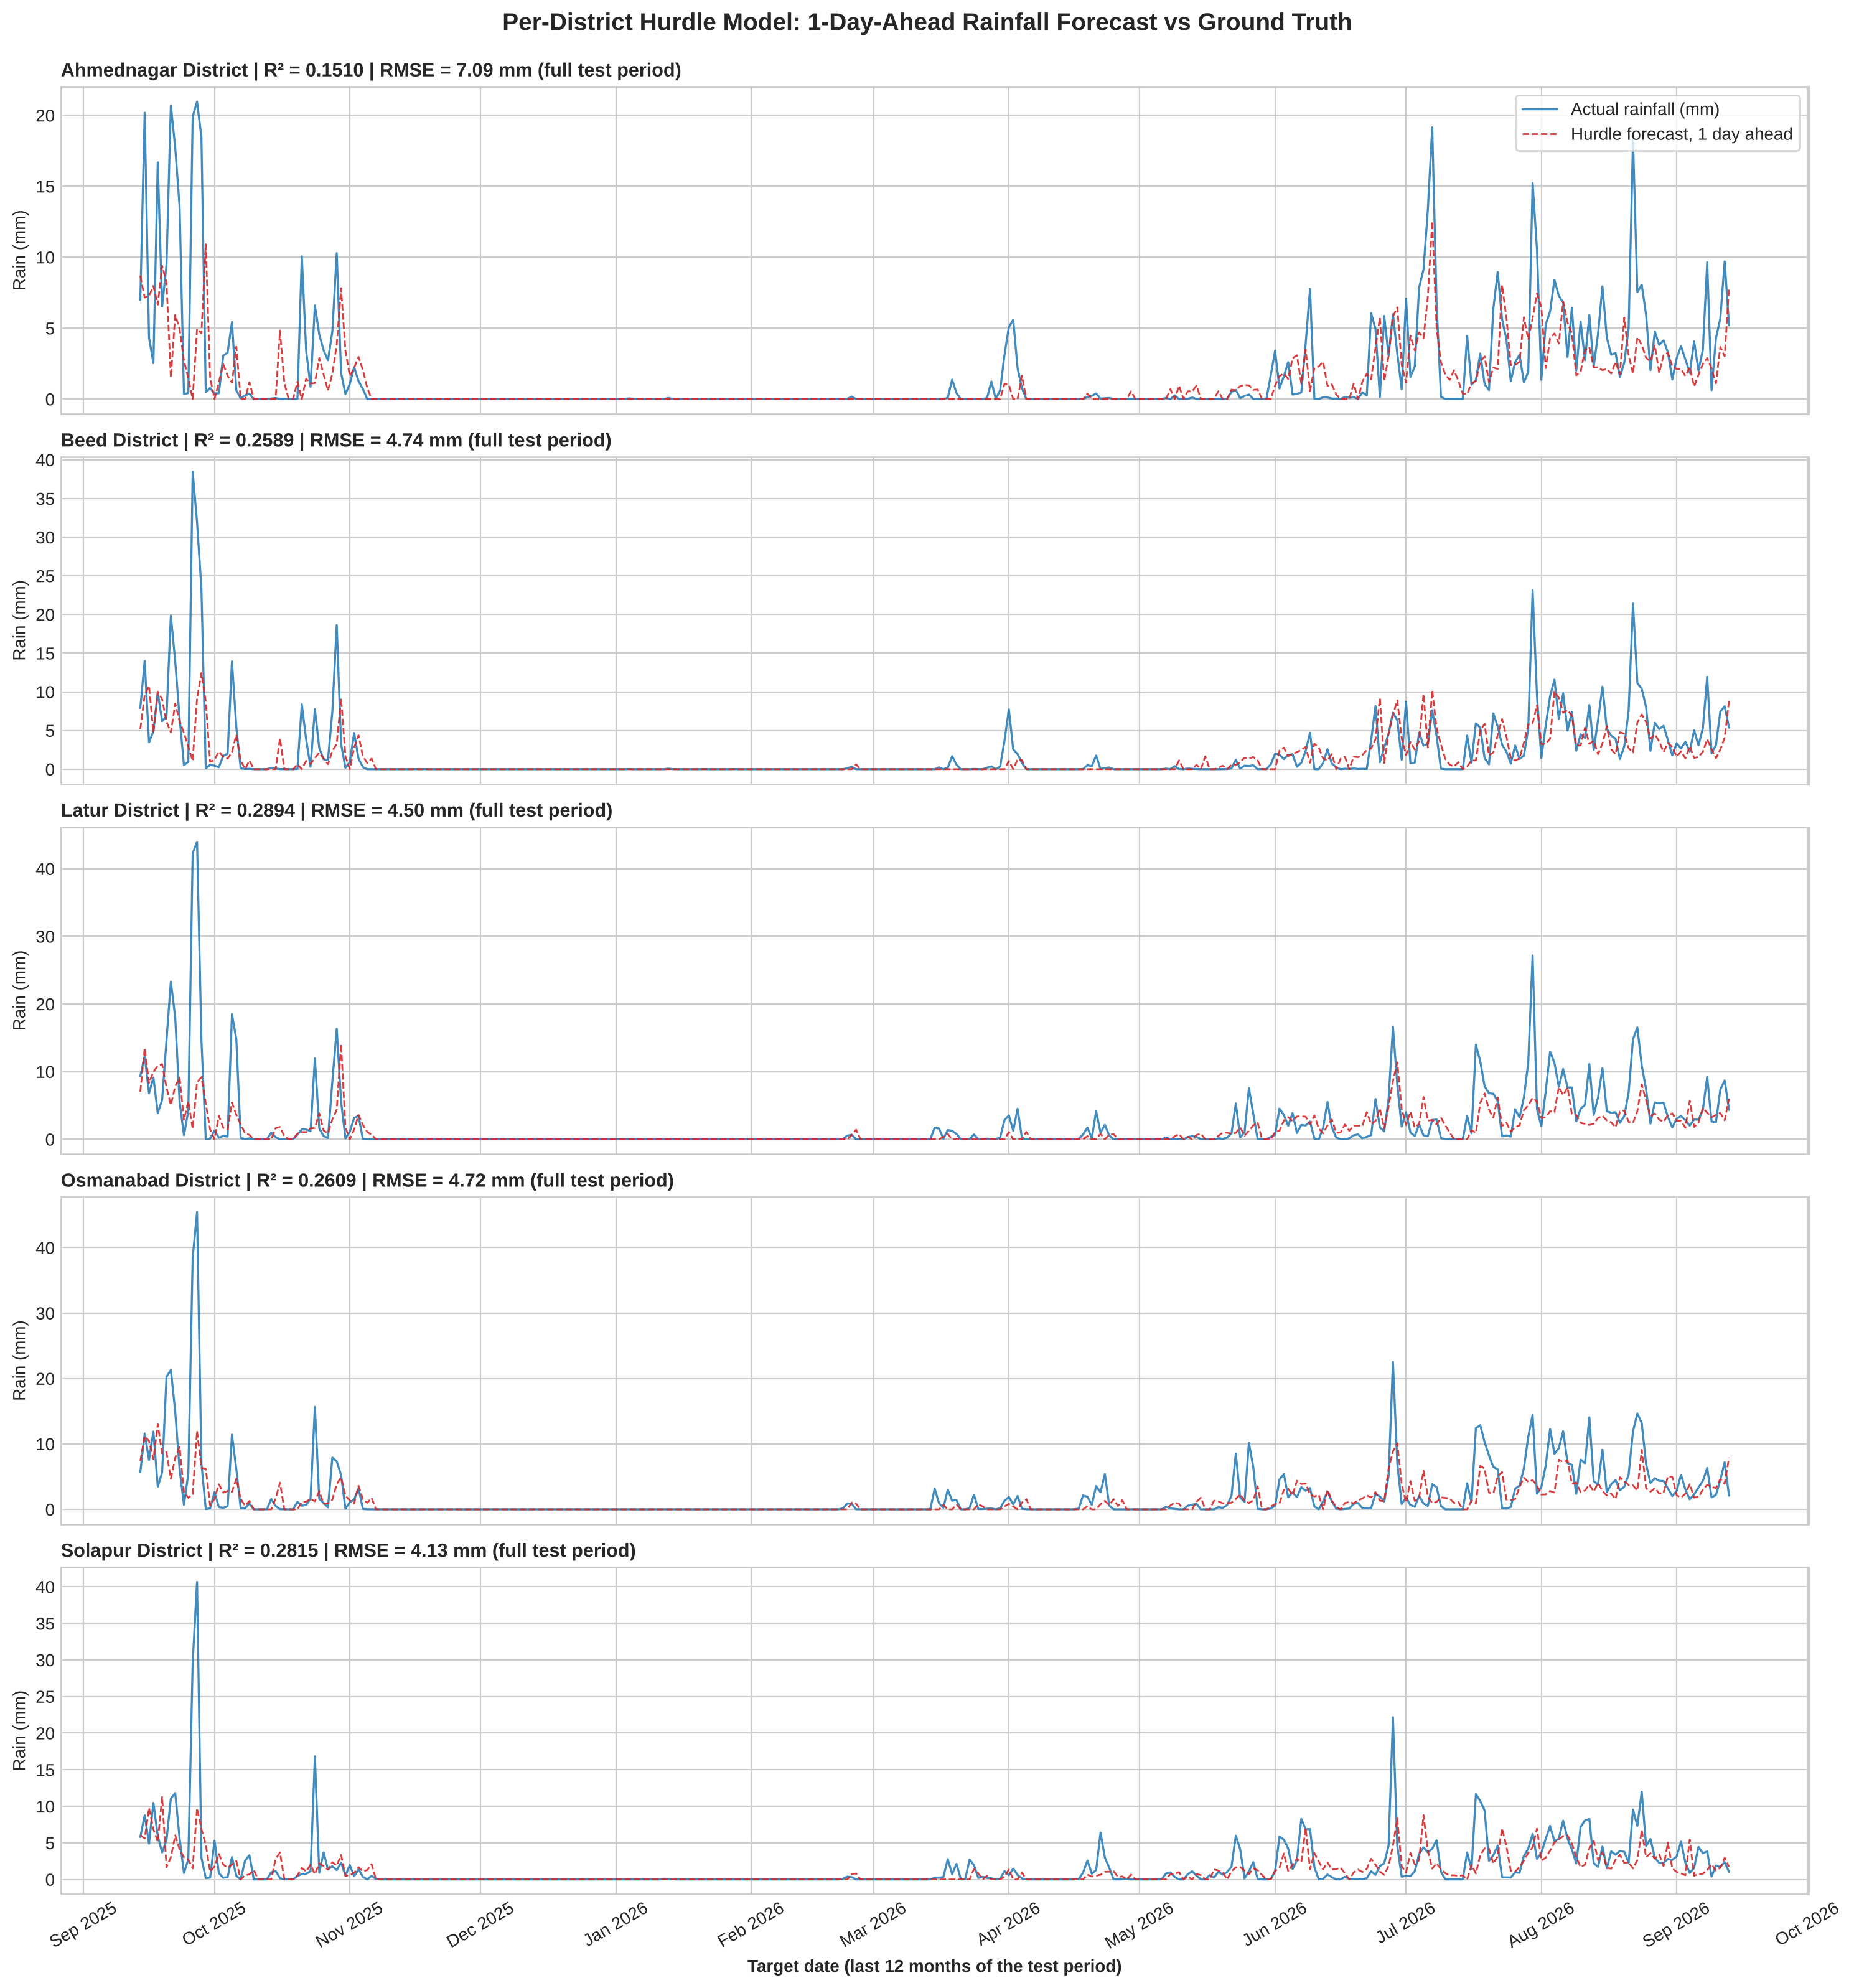
\includegraphics[width=0.97\textwidth,height=0.8\textheight,keepaspectratio]{hurdle_forecast_all_districts.png}
	\caption{Hurdle model: one-day-ahead rainfall forecast against observed rainfall for each district, September 2025 to September 2026. $R^2$ and RMSE in the panel titles are for the full test period (2022 onward).}
	\label{fig:hurdleall}
\end{figure}

\begin{figure}[H]
	\centering
	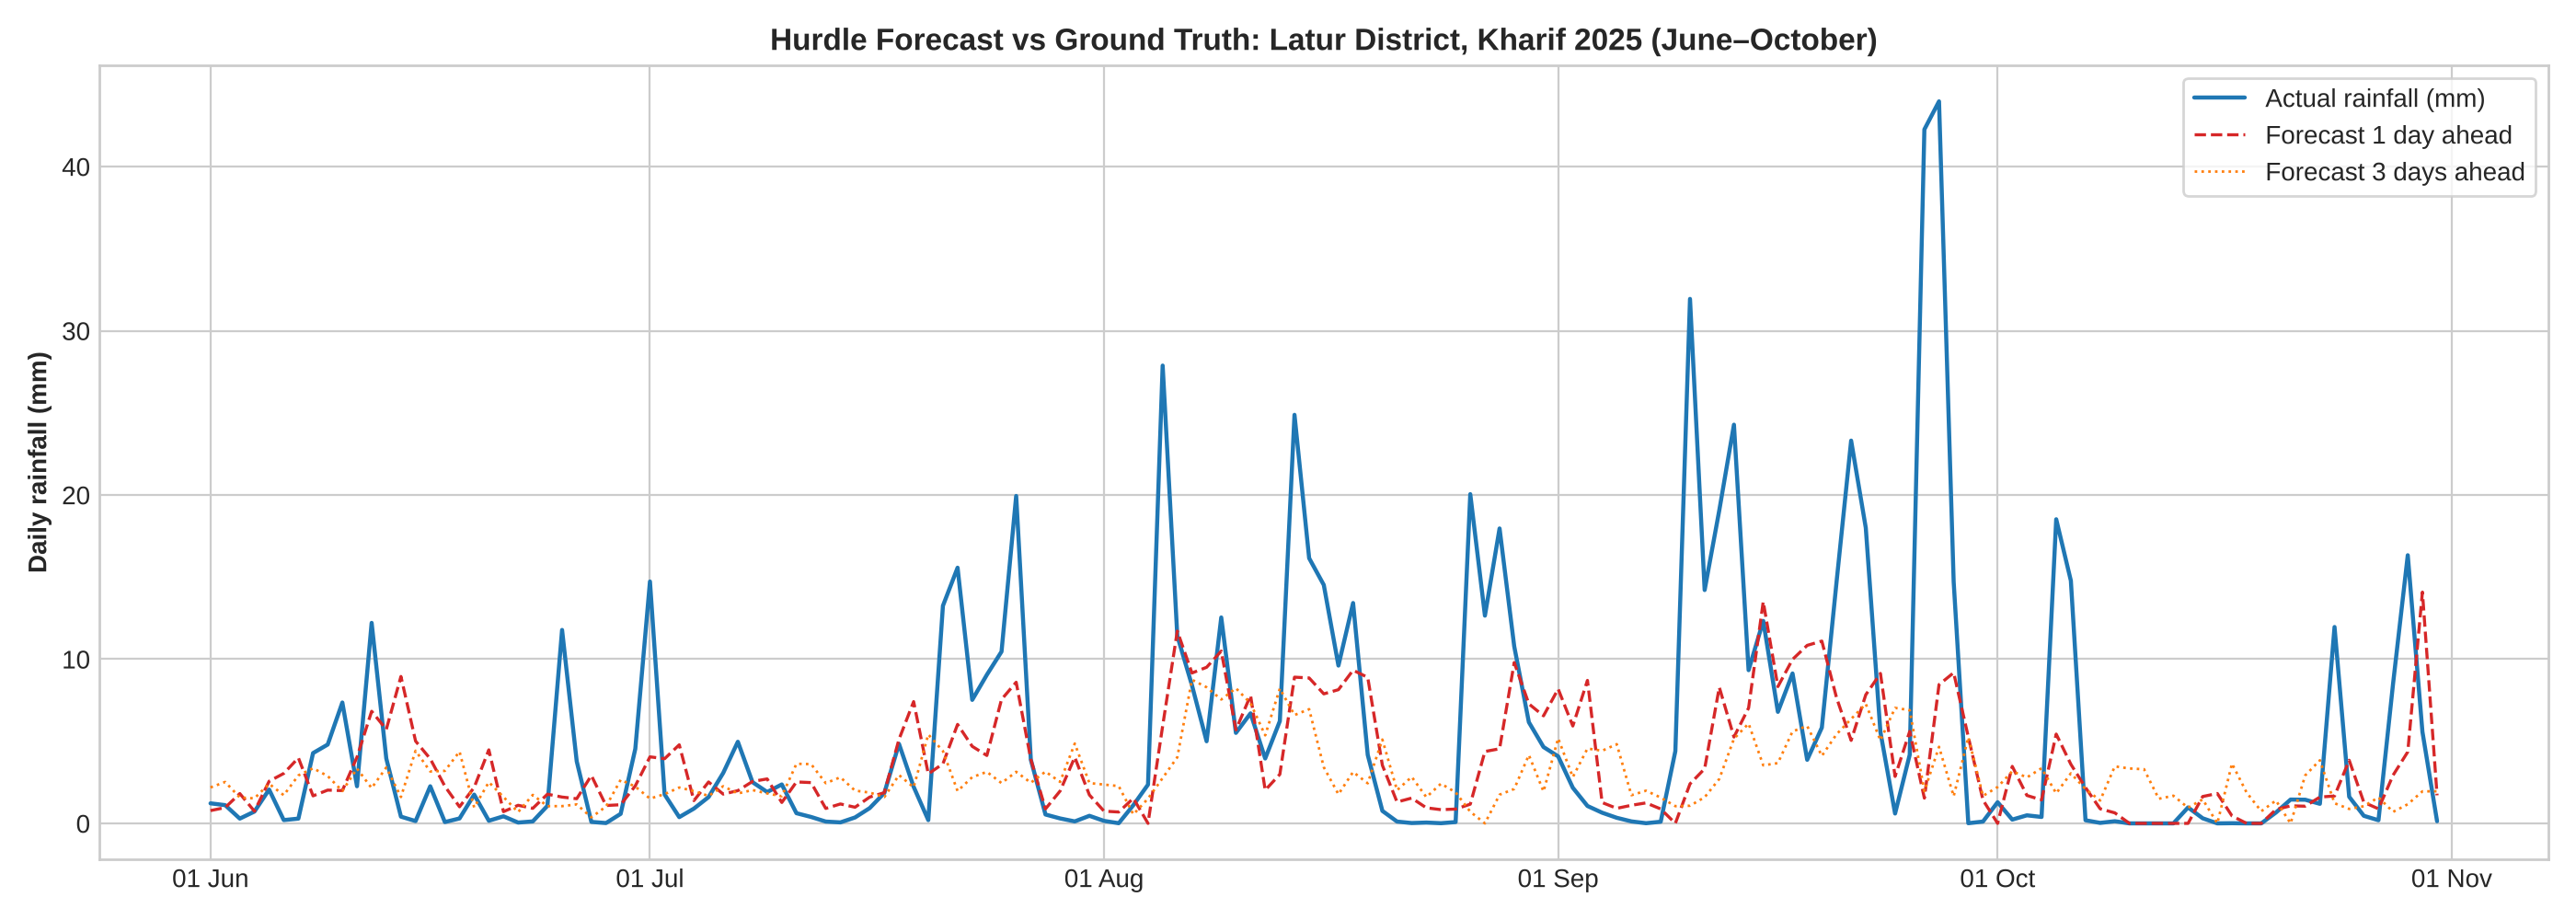
\includegraphics[width=\textwidth]{hurdle_latur_kharif2025.png}
	\caption{Hurdle model, Latur, Kharif 2025: forecasts one and three days ahead against observed rainfall.}
	\label{fig:hurdlelatur}
\end{figure}

What the model is good for in this system follows from these numbers. It gives a reliable short-range picture of whether the next one to three days are likely to stay dry, which is what decides whether a dry spell is continuing. Its gate also produces a \emph{probability of rain} that can be shown to users directly. It is not a season-long forecast; Stages 3--4 will combine it with the rainfall already observed in the season (Chapter~\ref{chap.conclusion}).

\section{Comparative study}
To test whether the hurdle model is the right choice, four other approaches were trained per district on the same weather data.

\subsection{LSTM network}
A Long Short-Term Memory network \cite{hochreiter1997long} reads a sequence one day at a time and keeps an internal memory, with gates that learn what to keep and what to forget. One model was trained per district.

\textbf{Inputs.} A window of the last 45 days, with 19 features per day: the 11 raw variables (rainfall, mean/maximum/minimum temperature, relative humidity, wind speed at 2\,m and 50\,m, surface pressure, solar radiation, dew point, cloud cover) and 8 rolling features (rainfall totals over 7, 14 and 30 days; 7-day means of humidity, solar radiation, wind, wind at 50\,m and cloud cover), plus day-of-year sine/cosine. Rainfall and wind speed were log-transformed, and all values scaled using the training period only.

\textbf{Architecture and training.} One LSTM layer of 128 units, followed by dense layers of 384 and 192 units with dropout 0.25, producing all 11 variables for the next 3 days in one output (33 numbers). Training used the Huber loss \cite{huber1964robust}, which behaves like squared error for small mistakes and like absolute error for large ones,
\begin{equation}
	\mathcal{L}_\delta(y,\hat{y}) =
	\begin{cases}
		\tfrac{1}{2}(y-\hat{y})^2 & \text{if } |y-\hat{y}| \le \delta,\\
		\delta\,|y-\hat{y}| - \tfrac{1}{2}\delta^2 & \text{otherwise,}
	\end{cases}
\end{equation}
with the Adam optimiser \cite{kingma2015adam} (learning rate $5\times10^{-4}$, batch size 16) and early stopping after 12 epochs without validation improvement. The data were split into training (to 2018), validation (2019--2021) and test (2022 onward). Figure~\ref{fig:loss} shows the loss curves for Latur.

\begin{figure}[H]
	\centering
	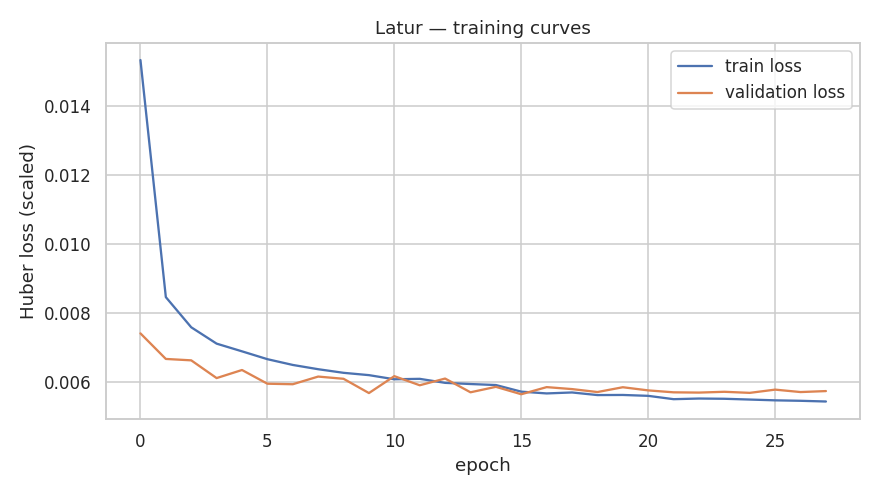
\includegraphics[width=0.65\textwidth]{loss_curve.png}
	\caption{Comparative LSTM: training and validation loss for Latur.}
	\label{fig:loss}
\end{figure}

\textbf{Results.} Because the LSTM forecasts all 11 variables, it also shows how forecastable the other variables are (Figure~\ref{fig:heatmap}, Table~\ref{tab:lstmdistrict}). Smooth variables are forecast well: temperature, humidity and dew point reach $R^2$ of 0.85--0.94 in every district. Rainfall is by far its weakest variable ($R^2$ 0.10--0.22): as Figures~\ref{fig:parity} and~\ref{fig:samples} show, its rainfall forecasts are squeezed towards small values and heavy rain is missed, exactly the behaviour described in Section~5.2.

\begin{figure}[H]
	\centering
	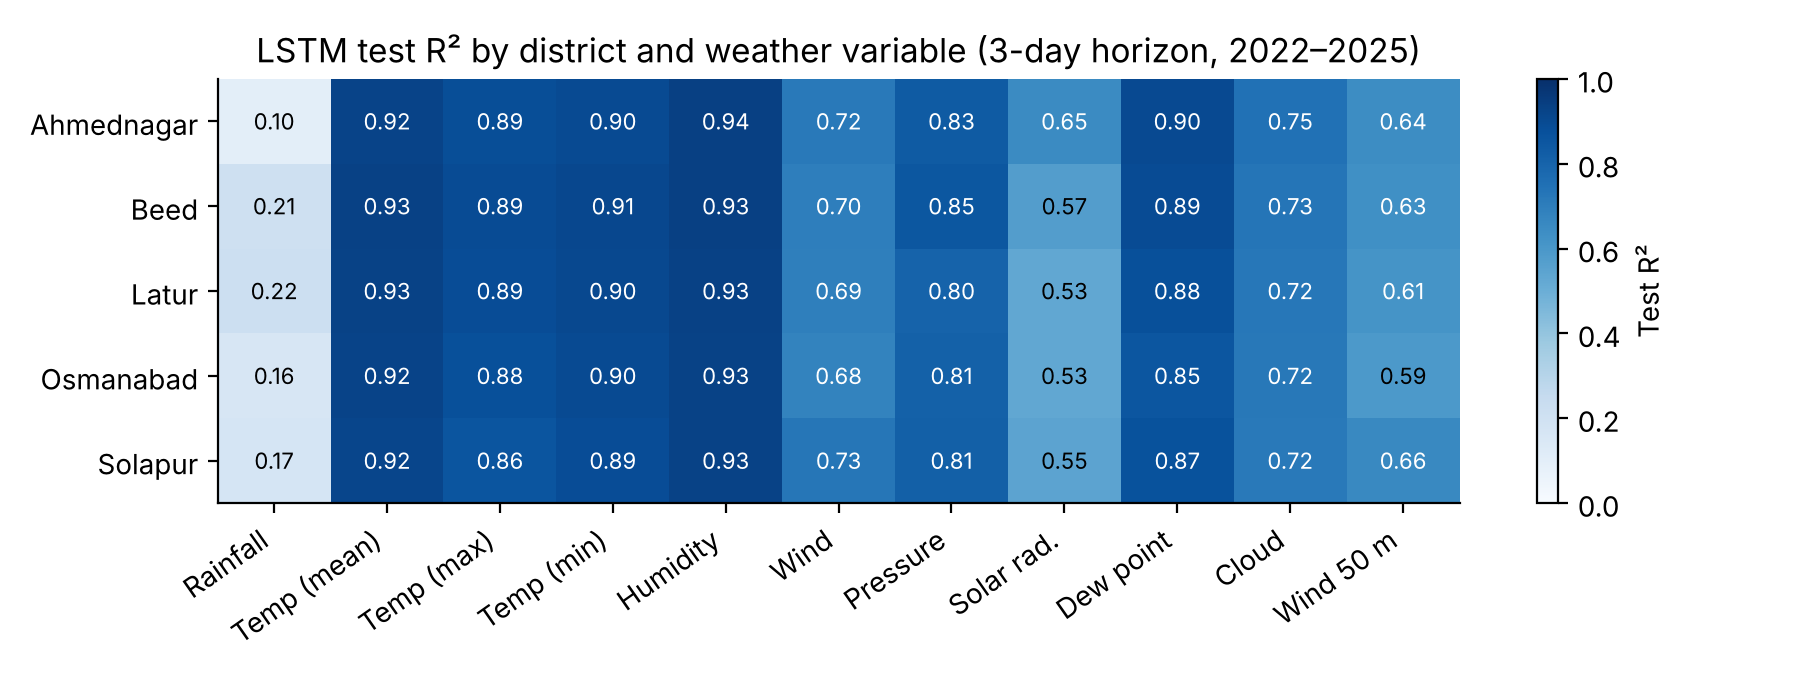
\includegraphics[width=\textwidth]{lstm_r2_heatmap.png}
	\caption{Comparative LSTM: test $R^2$ for every district and variable.}
	\label{fig:heatmap}
\end{figure}

\begin{table}[H]
	\centering
	\caption{Comparative LSTM: test results per district (2022 onward)}
	\label{tab:lstmdistrict}
	\begin{tabular}{lccc}
		\toprule
		\textbf{District} & \textbf{Average $R^2$ (11 variables)} & \textbf{Rainfall $R^2$} & \textbf{Rainfall MAE (mm)} \\
		\midrule
		Ahmednagar & 0.749 & 0.101 & 1.67 \\
		Beed & 0.750 & 0.209 & 1.68 \\
		Latur & 0.738 & 0.218 & 1.92 \\
		Osmanabad & 0.725 & 0.163 & 1.98 \\
		Solapur & 0.736 & 0.169 & 1.68 \\
		\bottomrule
	\end{tabular}
\end{table}

\begin{figure}[H]
	\centering
	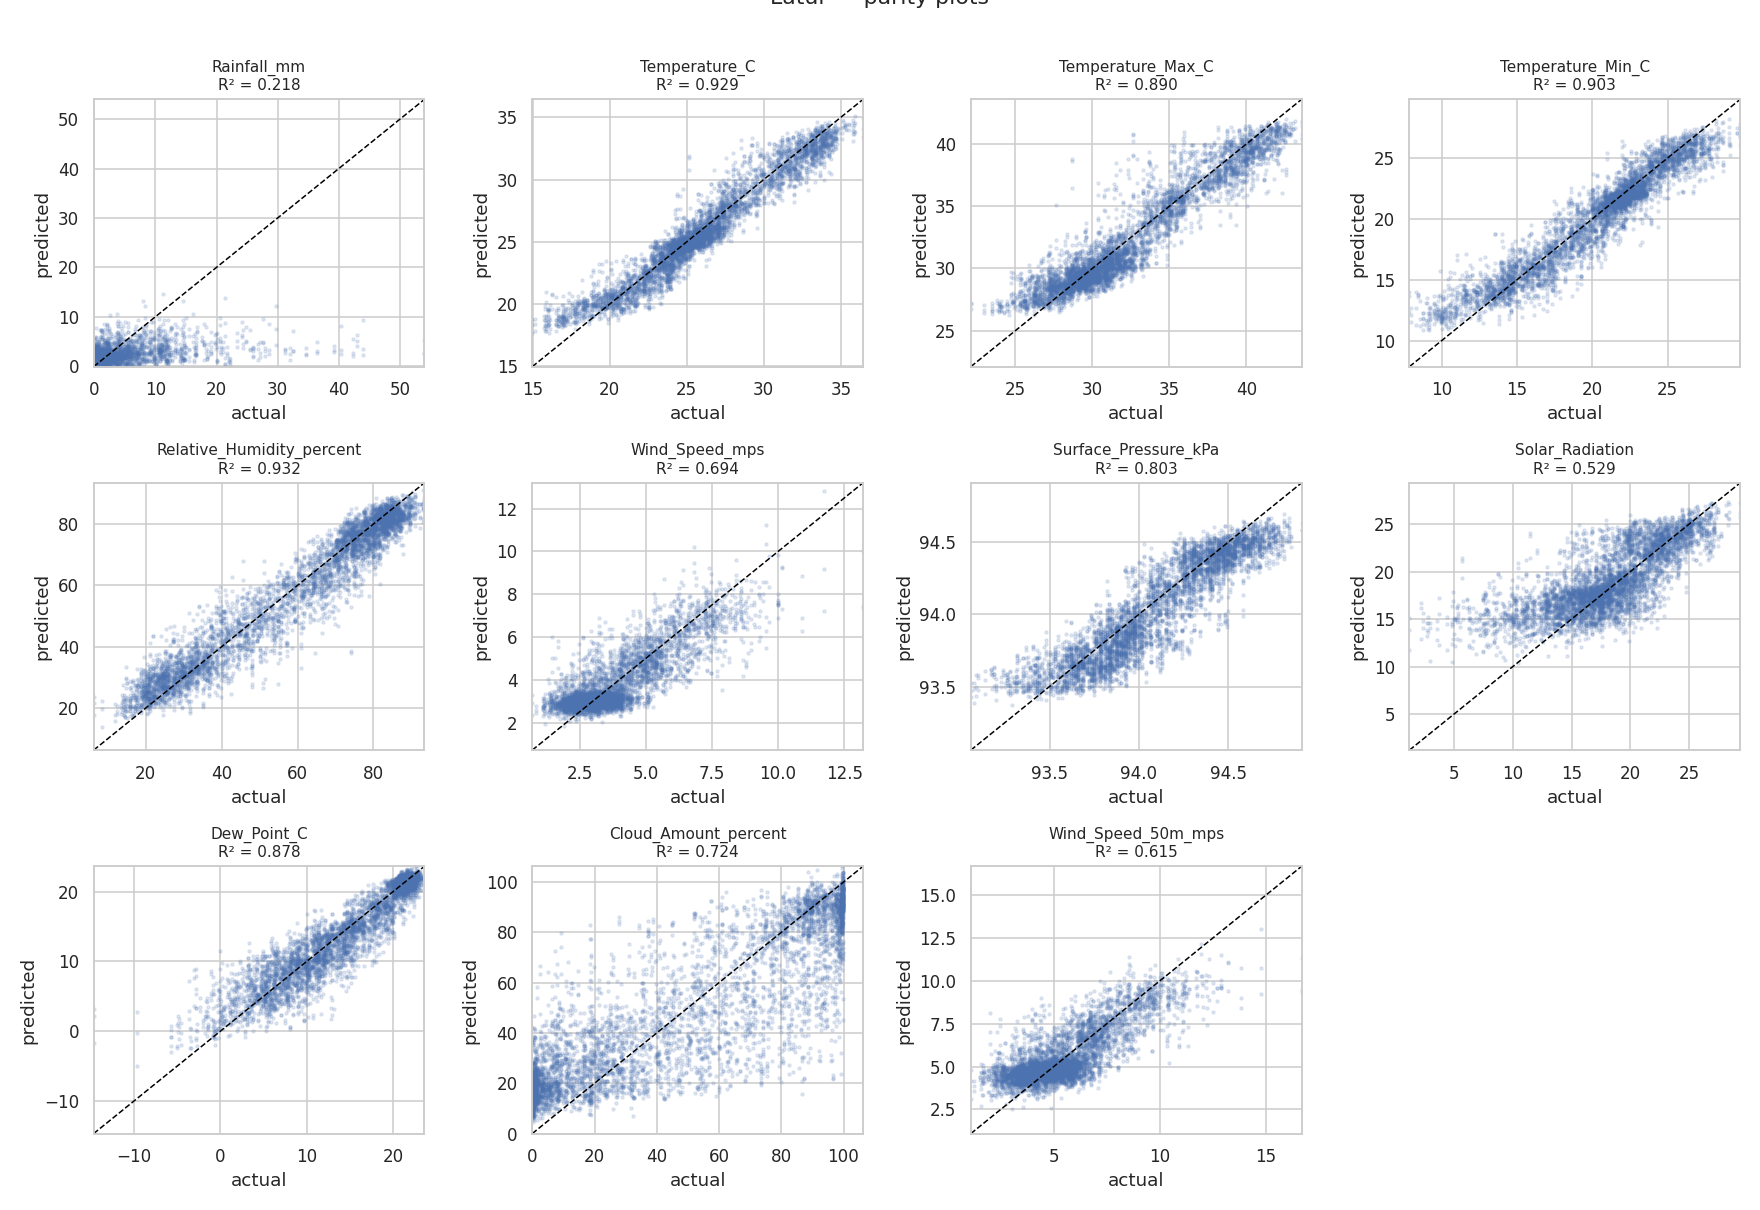
\includegraphics[width=0.9\textwidth]{parity_plots.png}
	\caption{Comparative LSTM, Latur: predicted against observed values on the test set. Temperature and humidity lie close to the diagonal; rainfall forecasts are compressed towards small values.}
	\label{fig:parity}
\end{figure}

\begin{figure}[H]
	\centering
	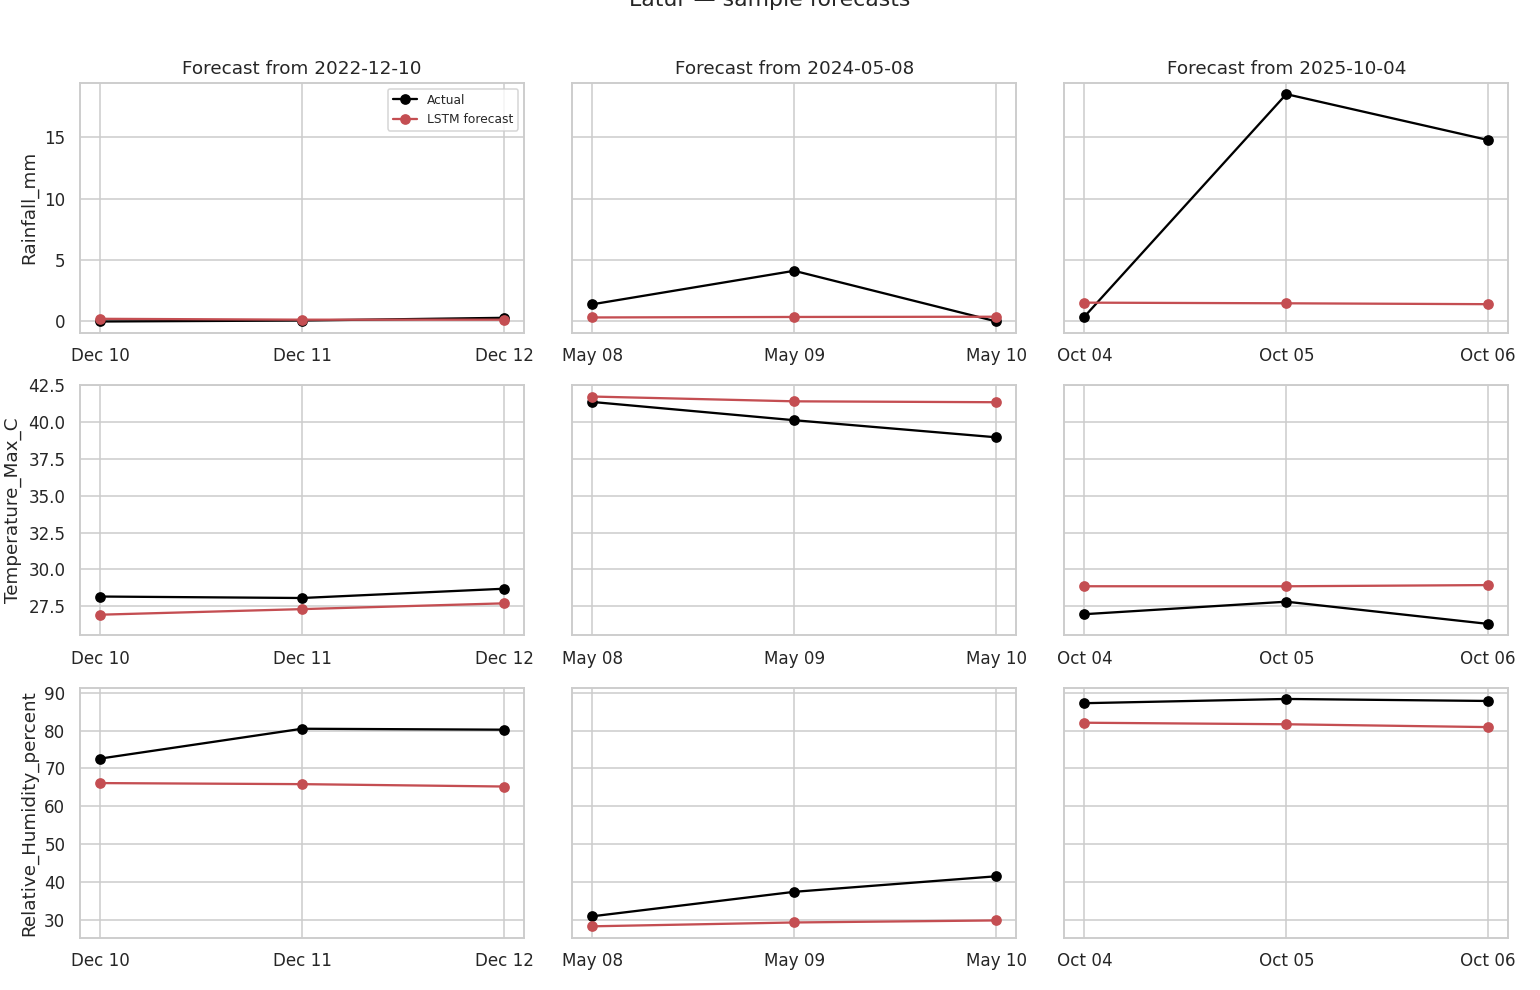
\includegraphics[width=0.9\textwidth]{sample_forecasts.png}
	\caption{Comparative LSTM, Latur: three sample 3-day forecasts. Temperature and humidity follow the observed trend; the heavy rain of 5--6 October 2025 is missed.}
	\label{fig:samples}
\end{figure}

\subsection{SARIMA}
A seasonal ARIMA model \cite{box2015time} was fitted per district as the statistical baseline. It forecasts the next value as a linear function of recent values, recent errors and the values one season earlier. It captures regular seasonality but assumes linear relations, so it struggles with the abrupt on/off behaviour of daily rain.

\subsection{XGBoost}
An XGBoost model \cite{chen2016xgboost} was trained per district on lagged and rolling-window weather features and seasonal terms. Gradient-boosted trees capture non-linear interactions, but used as a single regressor XGBoost treats rainfall as one continuous quantity and does not separate "will it rain?" from "how much?". The hurdle model uses the same family of learners but splits the problem in two.

\subsection{Temporal Fusion Transformer}
The TFT \cite{lim2021temporal} was trained as a multivariate, multi-horizon forecaster with attention over past time steps and learnt input selection. It is the most complex model in the study, and with about 9,500 daily rows per district it has comparatively little data to learn from. Like the LSTM, it predicts rainfall as a continuous value and has no explicit treatment of dry days.

\section{Comparison of results}
\subsection{Hurdle model and LSTM under the same protocol}
The LSTM and the hurdle model were both evaluated as genuine forecasts on the same test period (2022 onward), so their rainfall results can be compared directly (Table~\ref{tab:compare}, Figure~\ref{fig:rainskill}).

\begin{table}[H]
	\centering
	\caption{Rainfall test $R^2$: main hurdle model vs comparative LSTM}
	\label{tab:compare}
	\begin{tabular}{lccccc}
		\toprule
		& \multicolumn{4}{c}{\textbf{Hurdle (main)}} & \textbf{LSTM} \\
		\cmidrule(lr){2-5}
		\textbf{District} & \textbf{Day +1} & \textbf{Day +2} & \textbf{Day +3} & \textbf{Mean} & \textbf{Days +1..+3} \\
		\midrule
		Ahmednagar & 0.151 & 0.103 & 0.072 & 0.109 & 0.101 \\
		Beed & 0.259 & 0.190 & 0.147 & 0.199 & 0.209 \\
		Latur & 0.289 & 0.186 & 0.154 & 0.210 & 0.218 \\
		Osmanabad & 0.261 & 0.173 & 0.134 & 0.189 & 0.163 \\
		Solapur & 0.282 & 0.150 & 0.106 & 0.179 & 0.169 \\
		\bottomrule
	\end{tabular}
\end{table}

\begin{figure}[H]
	\centering
	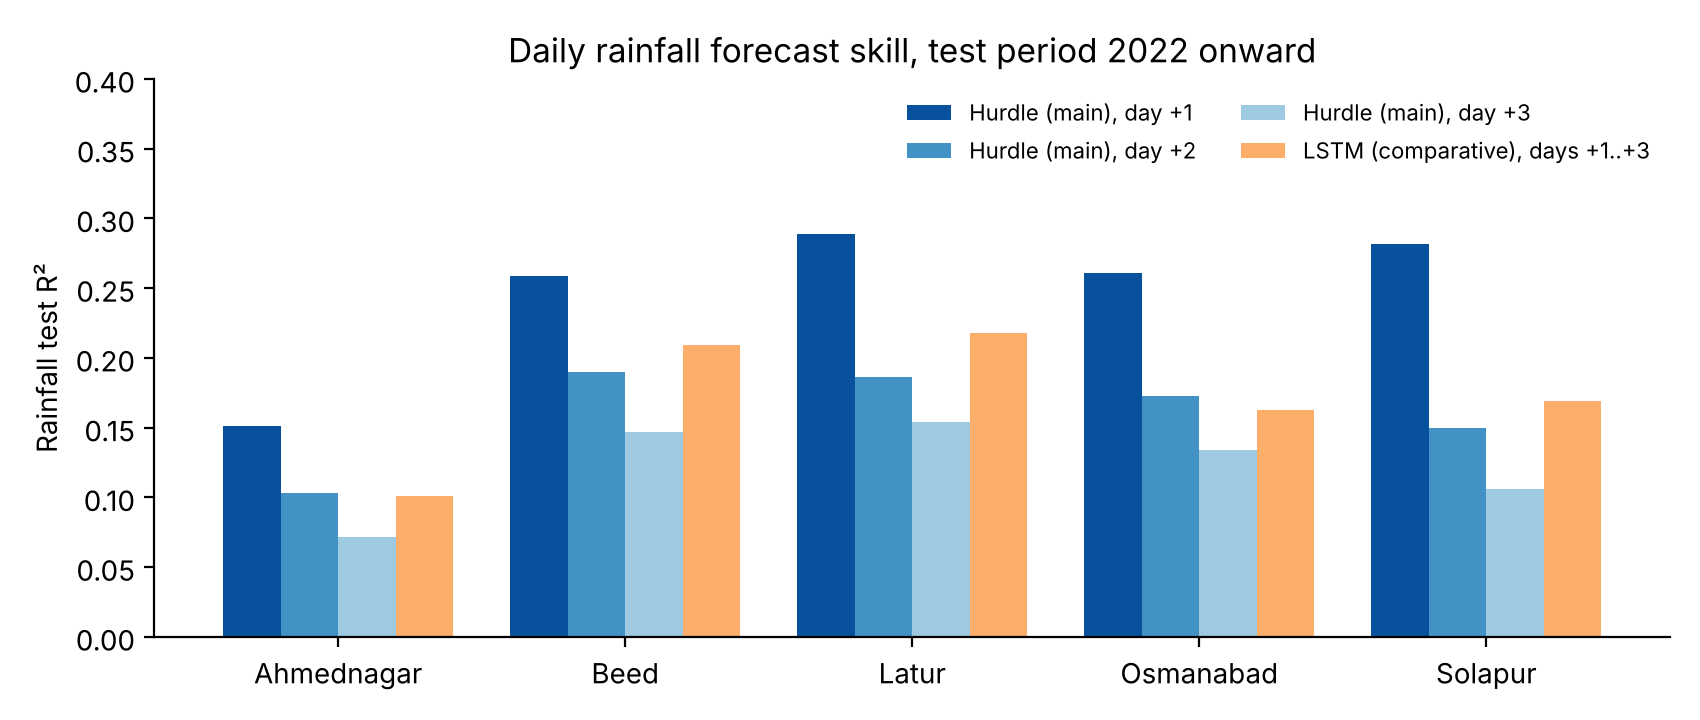
\includegraphics[width=0.9\textwidth]{rain_skill.png}
	\caption{Daily rainfall forecast skill of the main hurdle model at each horizon, compared with the LSTM.}
	\label{fig:rainskill}
\end{figure}

One day ahead, the hurdle model is better than the LSTM's rainfall forecast in every district. Averaged over the three days the two are close: the hurdle model is ahead in three districts and slightly behind in Beed and Latur.

\subsection{All five models as presented at the first review}
Table~\ref{tab:review} reproduces the test $R^2$ values presented at the first review. These numbers come from each model's own experimental set-up and are \textbf{not directly comparable}: the LSTM column averages all 11 variables (most of which are easy), the hurdle column is from the first, same-day version described in Section~\ref{sec:leak}, and the models differ in splits, targets and scaling. They are shown for completeness. Re-running SARIMA, XGBoost and TFT under the same protocol as Table~\ref{tab:compare} is part of the second-phase plan.

\begin{table}[H]
	\centering
	\caption{Test $R^2$ of the five models as presented at the first review (individual set-ups)}
	\label{tab:review}
	\begin{tabular}{lccccc}
		\toprule
		\textbf{District} & \textbf{Hurdle$^b$} & \textbf{SARIMA} & \textbf{XGBoost} & \textbf{LSTM$^a$} & \textbf{TFT} \\
		\midrule
		Ahmednagar & 0.923 & 0.432 & 0.303 & 0.749 & 0.511 \\
		Beed & 0.940 & 0.479 & 0.506 & 0.750 & 0.439 \\
		Latur & 0.945 & 0.592 & 0.590 & 0.738 & 0.500 \\
		Osmanabad & 0.885 & 0.544 & 0.549 & 0.725 & 0.439 \\
		Solapur & 0.787 & 0.512 & 0.509 & 0.736 & 0.372 \\
		\bottomrule
	\end{tabular}
	\\[2pt]
	\footnotesize $^a$ Average over all 11 variables. \quad $^b$ First (same-day) version; superseded by Table~\ref{tab:hurdle}.
\end{table}

\section{Why the hurdle model is the main model}
\begin{enumerate}
	\item \textbf{It is built for rainfall.} It separates "will it rain?" from "how much?", which matches how daily rainfall actually behaves (Section~5.2). None of the comparative models does this.
	\item \textbf{It gives the better next-day rainfall forecast} of the two models evaluated under the same protocol, in all five districts, and is on par with the LSTM over three days.
	\item \textbf{Its output is directly useful.} Besides the amount, the gate gives a probability of rain and a forecast of exactly 0\,mm on dry days, and it separates dry from rainy days correctly 81--88\% of the time up to three days ahead. This is what the dry-spell and onset rules in Stages 3--4 need.
	\item \textbf{It is light and easy to maintain.} It trains quickly on an ordinary CPU without a GPU, and is simple to version, retrain and monitor; it is the model run in the MLOps pipeline (Chapter~\ref{chap.7}).
	\item \textbf{It is easier to explain.} Gradient-boosted trees work with SHAP-style explanations \cite{lundberg2017unified}, which the project already plans for the yield stage.
\end{enumerate}
The comparative study remains useful: the LSTM shows that temperature, humidity and dew point can be forecast three days ahead with high accuracy, and these variables are available as supporting inputs if a later stage needs them.

\section{Summary}
A per-district, per-horizon two-stage hurdle model is the main forecasting model of the project. It forecasts daily rainfall 1--3 days ahead using only information available on the forecast day, with test $R^2$ of 0.15--0.29 one day ahead, falling to 0.07--0.15 at three days; its rain gate classifies 81--88\% of days correctly as dry or rainy. It gives better next-day rainfall forecasts than the LSTM, the comparative model evaluated under the same protocol. A comparative study of LSTM, SARIMA, XGBoost and TFT confirmed that models treating rainfall as a single continuous value struggle with its many dry days and rare heavy events, while the LSTM forecasts smoother variables such as temperature and humidity very well.
